\documentclass{standalone}

\usepackage{tikz}

\usetikzlibrary{calc}
\usetikzlibrary{math}

\begin{document}
  %noformat{
  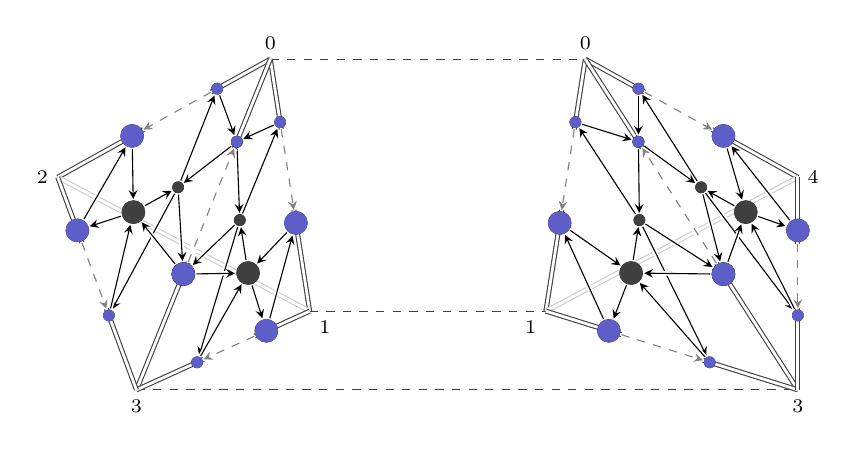
\begin{tikzpicture}
    \tikzstyle{v1} = [circle, outer xsep=0.5pt, fill, inner sep=1.5pt]
    \tikzstyle{v2} = [circle, outer xsep=0.5pt, fill, inner sep=3.0pt]
    \tikzstyle{unf} = [color=darkgray]
    \tikzstyle{frz} = [color=blue!60!darkgray!70]
    \tikzstyle{e} = [->, >={stealth}, preaction={draw=white, -, ultra thick}]
    \tikzstyle{h} = [dashed, color=gray, ->, >={stealth}]
    \tikzstyle{te} = [color=darkgray, double distance=1pt]

    \newcommand{\dummyquiver}[3]{
      \coordinate[v2] (A1)  at ($ (#1)!0.65!(#2) $) {};
      \coordinate[v1] (A2)  at ($ (#1)!0.25!(#2) $) {};
      \coordinate[v2] (B1)  at ($ (#1)!0.65!(#3) $) {};
      \coordinate[v1] (B2)  at ($ (#1)!0.25!(#3) $) {};
      \coordinate[v2] (C1)  at ($ (#2)!0.25!(#3) $) {};
      \coordinate[v1] (C2)  at ($ (#2)!0.65!(#3) $) {};
      \coordinate[v2] (v11) at ($ (#1)!0.65!(#2)!0.3!(#3) $) {};
      \coordinate[v1] (v21) at ($ (#1)!0.35!(#2)!0.3!(#3) $) {};

      \draw[h, preaction={draw=white, -, line width=2.3pt}] (A2) to[] (A1);
      \draw[h, preaction={draw=white, -, line width=2.3pt}] (B1) to[] (B2);
      \draw[h, preaction={draw=white, -, line width=2.3pt}] (C1) to[] (C2);

      \draw[e] (v11) -- (v21);
      \draw[e] (v11) -- ( C1);
      \draw[e] (v21) -- ( B1);
      \draw[e] (v21) -- ( C2);
      \draw[e] (v21) -- ( A2);
      \draw[e] ( B1) -- (v11);
      \draw[e] ( B2) -- (v21);
      \draw[e] ( C1) -- ( A1);
      \draw[e] ( C2) -- (v11);
      \draw[e] ( A1) -- (v11);
      \draw[e] ( A2) -- ( B2);

      \node[v2, frz] (A1n)  at (A1)  {};
      \node[v1, frz] (A2n)  at (A2)  {};
      \node[v2, frz] (B1n)  at (B1)  {};
      \node[v1, frz] (B2n)  at (B2)  {};
      \node[v2, frz] (C1n)  at (C1)  {};
      \node[v1, frz] (C2n)  at (C2)  {};
      \node[v2, unf] (v11n) at (v11) {};
      \node[v1, unf] (v21n) at (v21) {};
    }

    \tikzset{font=\scriptsize}


    \begin{scope}[shift={(3.7,0)}]
      \coordinate[label={ 90:{$0$}}] (v0t) at ($ (-2, 0) + ( 0.0, 2.1) $);
      \coordinate[label={330:{$1$}}] (v1t) at ($ (-2, 0) + ( 0.5,-1.1) $);
      \coordinate[label={180:{$2$}}] (v2t) at ($ (-2, 0) + (-2.7, 0.6) $);
      \coordinate[label={270:{$3$}}] (v3t) at ($ (-2, 0) + (-1.7,-2.1) $);

      \coordinate[label={ 90:{$0$}}] (v0b) at ($ ( 2, 0) + ( 0.0, 2.1) $);
      \coordinate[label={210:{$1$}}] (v1b) at ($ ( 2, 0) + (-0.5,-1.1) $);
      \coordinate[label={  0:{$4$}}] (v2b) at ($ ( 2, 0) + ( 2.7, 0.6) $);
      \coordinate[label={270:{$3$}}] (v3b) at ($ ( 2, 0) + ( 2.7,-2.1) $);

      \draw[dashed, darkgray] (v0t) -- (v0b);
      \draw[dashed, darkgray] (v1t) -- (v1b);
      \draw[dashed, darkgray] (v3t) -- (v3b);

      \draw[te,                 ] (v0t) -- (v1t);
      \draw[te,                 ] (v0t) -- (v2t);
      \draw[te,                 ] (v0t) -- (v3t);
      \draw[te, black!20!white  ] (v1t) -- (v2t);
      \draw[te,                 ] (v1t) -- (v3t);
      \draw[te,                 ] (v2t) -- (v3t);

      \draw[te,                 ] (v0b) -- (v1b);
      \draw[te,                 ] (v0b) -- (v2b);
      \draw[te,                 ] (v0b) -- (v3b);
      \draw[te, black!20!white  ] (v1b) -- (v2b);
      \draw[te,                 ] (v1b) -- (v3b);
      \draw[te,                 ] (v2b) -- (v3b);

      \dummyquiver{v0t}{v1t}{v3t}
      \dummyquiver{v0t}{v2t}{v3t}

      \dummyquiver{v0b}{v1b}{v3b}
      \dummyquiver{v0b}{v2b}{v3b}
    \end{scope}

  \end{tikzpicture}
  %}noformat
\end{document}
